\section{Radiation Damage Model}
The data collected with the CERN X-ray source  (\Cref{fig:DigiCurrentSummary}) was used to develop a model to predict an upper limit for the expected current increase in a 2S module under HL-LHC operating conditions. The model extends that proposed by Backhaus et al \cite{BackhausFeI4}, where the leakage current is attributed to the creation of leakage paths between source and drain via the inversion layer. The leakage paths are described as parasitic transistors, each with a transfer characteristic given by 
%created in the silicon along the \interface interface of the oxide
\begin{eqnarray}
I_D \approx 0 \,\,\,\,\,: \Neff < \Nthr \\
I_D \approx K_0~(\Neff - \Nthr)^2 \,\,\,\,\,: \Neff \ge \Nthr ,
\label{eq:TransferCharacteristic_ParasiticTransistors}
\end{eqnarray}
where $\Neff$ is the effective number of charges located in the inversion layer created by the build-up of positive charge in the oxide, $\Nthr$ is the threshold number of charges required to activate the transistor, and ${K_0}$ is a proportionality constant.
\begin{figure}[htbp]
\centering
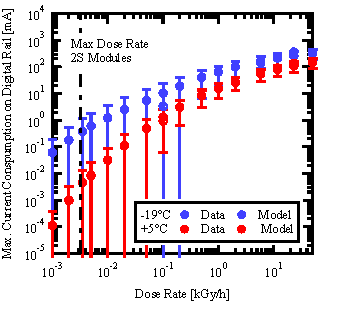
\includegraphics[width=0.8\linewidth]{Figures/ModelPrediction_CurrentConsumption.pdf}
\vspace*{-5mm}
\caption{The size of reconstructed clusters in strips (635 $\mu$m
strip pitch) for both readout coordinates of the central detector.}
\label{fig:ModelComparison_CurrentIncrease}
\end{figure}

The effective number of charges in the transistor can be expressed as
\begin{equation}
\Neff = \Not - \Nit. 
\label{eq:Neff}
\end{equation}
where ${\Not}$ and ${\Nit}$ are the positive trapped charge and interface traps created \cite{BarnabyTIDeffects} when electron-hole pairs (ehps) generated by ionization interact with existing defects and impurities in the oxide. Holes that survive initial prompt recombination may be trapped by deep traps as they move throughout the oxide; while those not trapped by defect sites are free to interact with hydrogen-containing defects ($D^{'}H$) introduced in the oxide during its growth. The simplest of these interactions releases a proton ($H^+$) from the defect site. Interface traps are created when a proton produced by such a reaction reaches the \interface interface and removes a hydrogen molecule ($H_2$) from a dangling bond (${SiH}$); creating an interface trap.
% Trapped holes, i.e. trapped positive charge $\Not$, have a finite probability of escaping from these traps depending on the energy level(s) of the traps and the temperature of the device during irradiation. 

The rate of creation of trapped positive charge in the oxide can therefore be given by
\begin{equation}
\dot N_{\mbox{\tiny{OT}}} = f_{\mbox{\tiny{OT}}}k_0\,\dot D\,(\NotMax - \Not)- \Rot\,\Not ,
\label{eq:Not_TrappingRate}
\end{equation}
where $f_{\mbox{\tiny{OT}}}$ is a deep trap's hole trapping probability, ${k_0}$ is a constant proportional to the introduction rate of holes in the oxide, $\Rot$ is the de-trapping rate of holes, $\NotMax$ is the maximum number of deep trapping sites in the oxide, and ${\dot D}$ is the dose rate. In addition, the rate of proton release can expressed as 
\begin{equation}
\dot p = f_p\,(k_0\,\dot D - \dNot)\,(N_p - p),
\label{eq:Proton_ReleaseRate}
\end{equation}
where ${f_p}$ is a hydrogen-containing defect's proton trapping a hole, ${(k_0\,\dot D - \dNot)}$ describes the number of holes available to participate in this process, and ${N_p}$ is the maximum number of available hydrogen-containing defects in the oxide. Finally, the rate of interface trap creation can be modeled by 
\begin{equation}
\dot N_{\mbox{\tiny{IT}}} = f_I\,(N_{\mbox{\tiny{SiH}}} - N_{\mbox{\tiny{IT}}}) \dot p, 
\label{eq:Nit_TrappingRate_0}
\end{equation}
 where ${f_I}$ is the probability that an available dangling bond captures the free proton, and $\NitMax$ is the number of hydrogen-passivated dangling bonds present in the un-irradiated oxide. An analytical description for the number of fixed positive charges $\Not$ and interface traps $\Nit$ created during an irradiation can be found by solving the system of coupled differential equations described by ~\Cref{eq:Not_TrappingRate,eq:Proton_ReleaseRate,eq:Nit_TrappingRate_0}. The solution for the case where the irradiation starts at ${t=0}$ is given by
\begin{eqnarray}
\Nit = \NitMax\,[1 - e^{- p(t)}] \\ 
\Not = \NotMax\,\frac{\Fot k_0 \dot D}{\Fot k_0 \dot D + \Rot}\,[1 - e^{-(\Fot k_0 \dot D + \Rot)t}] \\
p(t) = f_I\,N_p[ 1 - e^{-f_p k_0\,\dot D\,t + f_p\,\Not(t)} ].
\label{eq:Solution_DifferentialEquations}
\end{eqnarray}

A simultaneous fit of the parametrized damage model to the data collected for each set of four chips irradiated at $-19$\deg and $5$\deg was used to extract the dose-rate dependence of the model parameters. The predicted current increase at the expected HL-LHC dose rate and $-19$\deg, shown in \Cref{fig:ModelComparison_CurrentIncrease}, is believed to be a conservative upper limit on the current increase expected in 2S modules due to radiation induced leakage in the CBC3s. 

%(e.g. oxygen vacancies in the oxide bulk and/or hydrogen passivated dangling  bonds at the \interface interface).
% and the total (digital) leakage current of the CBC3 when exposed to ionizing radiation can be written as 
% \begin{equation}
% \Ileak = \IpreIrrad + K~(\Not - \Nit - \Nthr)^2 \,\,\mbox{for}\,\, \Neff \ge \Nthr , 
% \label{eq:LeakageCurrent_CBC3}
% \end{equation} 
% where $K$ is a new proportionality constant that takes into account that the total leakage current measured in the CBC3 is the sum of the additional current flowing through the many thousands of transistors that make up the digital logic of the CBC3.


% In the case of NMOS transistors (of the type used in the CBC3) the build-up of positive charge in the oxide results in positive charge ($\Not$) build-up, whilst the creation of interface traps ($\Nit$) at the \interface interface results in a negative space charge. Therefore the effective number of charges in the transistor can be expressed as
% \begin{equation}
% \Neff = \Not - \Nit. 
% \label{eq:Neff}
% \end{equation}
% and the total (digital) leakage current of the CBC3 when exposed to ionizing radiation can be written as 
% \begin{equation}
% \Ileak = \IpreIrrad + K~(\Not - \Nit - \Nthr)^2 \,\,\mbox{for}\,\, \Neff \ge \Nthr , 
% \label{eq:LeakageCurrent_CBC3}
% \end{equation} 
% where $K$ is a new proportionality constant that takes into account that the total leakage current measured in the CBC3 is the sum of the additional current flowing through the many thousands of transistors that make up the digital logic of the CBC3.

% Positive trapped charge and interface traps at the \interface interface are created in a CMOS circuit exposed to ionizing radiation when electron-hole pairs (ehps) generated by the ionizing radiation interact with existing defects and impurities (e.g. oxygen vacancies in the oxide bulk and/or hydrogen passivated dangling  bonds at the \interface interface).
%which is dependent on the energy level(s) of the deep traps located in the oxide and the temperature at which the irradiation takes place.

%\cite{BarnabyTIDeffects}
% Holes not trapped by defect sites are free to interact with hydrogen containing defects ($D^{'}H$) introduced in the oxide during its growth. The simplest of these interactions acts to release a proton ($H^+$) from the defect site with a rate of proton release given by
% \begin{equation}
% \dot p = f_p\,(k_0\,\dot D - \dNot)\,(N_p - p),
% \label{eq:Proton_ReleaseRate}
% \end{equation}
% where ${f_p}$ is a hydrogen containing defect's proton trapping a hole, ${(k_0\,\dot D - \dNot)}$ describes the number of holes available to participate in this process, and ${N_p}$ is the maximum number of available hydrogen containing defects in the oxide. Interface traps are created when a proton produced by such a reaction reaches the \interface interface. The rate of interface trap creation can therefore be written as
% \begin{equation}
% \dot N_{\mbox{\tiny{IT}}} = f_I\,(N_{\mbox{\tiny{SiH}}} - N_{\mbox{\tiny{IT}}}) \dot p, 
% \label{eq:Nit_TrappingRate_0}
% \end{equation}
%  where ${f_I}$ is the probability that an available dangling bond captures the free proton, and $\NitMax$ is the number of hydrogen passivated dangling bonds present in the un-irradiated oxide.

% An analytical description for the number of fixed positive charges $\Not$ and interface traps $\Nit$ created during an irradiation can be found by solving the system of coupled differential equations described by ~\Cref{eq:Not_TrappingRate,eq:Proton_ReleaseRate,eq:Nit_TrappingRate_0}. The solution for the case where the irradiation starts at ${t=0}$ is given by
% \begin{eqnarray}
% \Nit = \NitMax\,[1 - e^{- p(t)}] \\ 
% \Not = \NotMax\,\frac{\Fot k_0 \dot D}{\Fot k_0 \dot D + \Rot}\,[1 - e^{-(\Fot k_0 \dot D + \Rot)t}] \\
% p(t) = f_I\,N_p[ 1 - e^{-f_p k_0\,\dot D\,t + f_p\,\Not(t)} ].
% \label{eq:Solution_DifferentialEquations}
% \end{eqnarray}
% This can then be used to fit the increase in the leakage current ${\Ileak - \IpreIrrad}$ measured at different dose rates and temperatures with the CERN X-ray source. The dose rate dependence of the model parameters in this model are used to predict the expected current increase at dose rates beyond those measured here, as shown in \Cref{fig:ModelComparison_CurrentIncrease}.


% The damage model developed by Backhaus et. al attributes the leakage current increase of linear NMOS transistors to the creation of leakage paths between source and drain via the inversion layer created in the silicon along the \interface interface of the STI. 
% \begin{figure}[!htbp]
%  \centering
%   \subfloat[][Pre-irradiation.]
%   {
%     \includegraphics[width=0.25\columnwidth]{./Fig/NMOS_PreIrrad.eps}
%     \label{fig:NMOS_preIrrad}
%   }
%   \quad
%   \subfloat[][Post-irradiation (gate removed).]
%   {
%     \includegraphics[width=0.25\columnwidth]{./Fig/NMOS_Irrad.eps}
%     \label{fig:NMOS_Irrad}
%   }
%  \caption[Linear NMOS transistor before and after exposure to ionizing radiation.]{Top views of a linear NMOS transistor before (left) and after (right) exposure to ionizing radiation. The fixed positive charge built up in the STI and the corresponding inversion layer created in the channel of the transistor are also shown.}
%  \label{fig:NMOS}
% \end{figure} 
% The leakage current paths are described in \cite{BackhausFeI4} as parasitic with a transfer characteristic 
% \begin{eqnarray}
% I_D \approx 0 \,\,\,\,\,: \Neff < \Nthr \\
% I_D \approx K_0~(\Neff - \Nthr)^2 \,\,\,\,\,: \Neff \ge \Nthr ,
% \label{eq:TransferCharacteristic_ParasiticTransistors}
% \end{eqnarray}
% where $\Neff$ is the effective number of charges located in the inversion layer created in the silicon by the build-up of positive charge in the STI, $\Nthr$ is the threshold number of charges required to activate the transistor, and ${K_0}$ is a proportionality constant containing the widths, lengths, oxide capacitance and the mobility of the minority charge carriers in the channel of the transistor. In the case of NMOS transistors (of the type used in the CBC3) the build-up of positive charge in the STI results in positive charge, whilst the creation of interface traps at the \interface interface results in a negative space charge. Therefore the effective number of charges in the transistor can be expressed as
% \begin{equation}
% \Neff = \Not - \Nit. 
% \label{eq:Neff}
% \end{equation}

% Therefore the total (digital) leakage current of the CBC3 when exposed to ionizing radiation can be written as 
% \begin{equation}
% \Ileak = \IpreIrrad + K~(\Not - \Nit - \Nthr)^2 \,\,\mbox{for}\,\, \Neff \ge \Nthr , 
% \label{eq:LeakageCurrent_CBC3}
% \end{equation} 
% where $K$ is a new proportionality constant that takes into account that the total leakage current measured in the CBC3 is the sum of the additional current flowing through the many thousands of transistors that make up the digital logic of the CBC3 and ${\Not,\Nit}$ are the solutions to the rate equations derived for the build-up of positive fixed charge and interface traps derived in \Cref{subsec:Not,subsec:Nit}.

% %re-phrase this... needs thinking (want to say why this effect is present only in NMOS)
% % The space charge in the STI is always positive and therefore in PMOS transistors this transistor channel is closed by the radiation induced space charge. Thus the leakage current increase is only observed in NMOS transistors.

% Finding an analytical description for the number of fixed positive charges $\Not$ and interface traps $\Nit$ created during an irradiation requires solving the system of coupled differential equations described by ~\Cref{eq:Not_TrappingRate,eq:Proton_ReleaseRate,eq:Nit_TrappingRate_0}. The solution for the case where the irradiation starts at ${t=0}$ is given by
% \begin{eqnarray}
% \Nit = \NitMax\,[1 - e^{- p(t)}] \\ 
% \Not = \NotMax\,\frac{\Fot k_0 \dot D}{\Fot k_0 \dot D + \Rot}\,[1 - e^{-(\Fot k_0 \dot D + \Rot)t}] \\
% p(t) = f_I\,N_p[ 1 - e^{-f_p k_0\,\dot D\,t + f_p\,\Not(t)} ],
% \label{eq:Solution_DifferentialEquations}
% \end{eqnarray}
% (the details of the solution are provided in the appendix). \Cref{eq:LeakageCurrent_CBC3,eq:Solution_DifferentialEquations} can then be used to fit the increase in the leakage current ${\Ileak - \IpreIrrad}$ measured at different dose rates and temperatures with the CERN X-ray source. If the fit can also be used to establish the dose rate dependence of the model parameters then this model can be used to predict the expected current increase at dose rates beyond those measured here. The following section describes how this was achieved using the results from the X-ray irradiation of the CBC3s at temperatures of ${-19}$\deg/5\deg and a bias voltage of $1.25\,$\volt. 

% % \begin{figure}[htbp]
% % \centering
% % 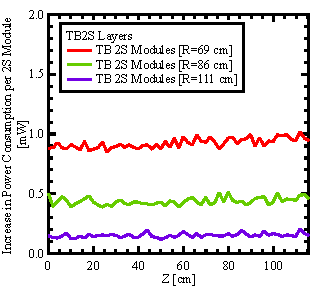
\includegraphics[width=0.8\linewidth]{Figures/ModelPrediction_PowerConsumption.pdf}
% % \caption{The size of reconstructed clusters in strips (635 $\mu$m
% % strip pitch) for both readout coordinates of the central detector.}
% % \label{fig:ModelPredictionPower}
% % \end{figure}

